\documentclass[12pt]{article}

% BibTeX setup
\usepackage[backend=bibtex, bibstyle=alphabetic, citestyle=alphabetic]{biblatex}
\bibliography{references}

% \usepackage[english]{babel} % English
\usepackage[ngerman]{babel} % German

\usepackage{enumitem} % Package for handling of lists
\setlist{noitemsep}   % No separating whitespace between list items.

% Standard packages for math-related things.
\usepackage{amsmath}
\usepackage{amssymb}
\usepackage{amsthm}

\usepackage{mathtools}

\usepackage{graphicx} % to include graphics with \includegraphics[options]{imagefile}

\usepackage{tikz}
\usepackage{pgfplots}

% Hyperref is great, but sometimes there are problems if packages are loaded before or after hyperref. Check the documentation.
\usepackage{hyperref} % For PDF links, toc, etc.

% Formatting of paragraphs
\parindent 0cm                     % No intendation at the beginning of a paragraph
\parskip1.5ex plus0.5ex minus0.5ex % Vertical space between two paragraphs


%%%%%%%%%%%%%%%%%%%%%%%%%%%%%%%%%%%%%%%%%%%%%%%%%%%%%%%%%%%%%%%%%%%%%%%%%%%%%%%%
% Theorem and style definitions (for amsthm). For details see
% https://en.wikibooks.org/wiki/LaTeX/Theorems
%%%%%%%%%%%%%%%%%%%%%%%%%%%%%%%%%%%%%%%%%%%%%%%%%%%%%%%%%%%%%%%%%%%%%%%%%%%%%%%%

\theoremstyle{plain} % Usual style for theorems, etc.

% All numbered with the same counter (theorem).
% \newtheorem{theorem}{Theorem}[section] % This uses numbering SECTION.COUNT instead of COUNT. Useful in longer documents.
\newtheorem{theorem}{Satz} % Number linearly (no SECTION prefix).
% Usage: \newtheorem{environmentname}[counter]{displayedtext}
\newtheorem{proposition}[theorem]{Proposition}
\newtheorem{lemma}[theorem]{Lemma}
\newtheorem{corollary}[theorem]{Korollar}
\newtheorem*{lemma*}{Lemma} % not numbered.

\theoremstyle{definition} % Usual style definitions.
\newtheorem{definition}[theorem]{Definition}
\newtheorem*{definition*}{Definition}

\theoremstyle{remark} % Usual style definitions.
\newtheorem{remark}[theorem]{Remark}


%%%%%%%%%%%%%%%%%%%%%%%%%%%%%%%%%%%%%%%%%%%%%%%%%%%%%%%%%%%%%%%%%%%%%%%%%%%%%%%%
% Some commands
%%%%%%%%%%%%%%%%%%%%%%%%%%%%%%%%%%%%%%%%%%%%%%%%%%%%%%%%%%%%%%%%%%%%%%%%%%%%%%%%

\newcommand{\IN}{\mathbb{N}} % blackboard bold N for natural numbers
\newcommand{\IR}{\mathbb{R}} % blackboard bold R for real numbers
\newcommand{\IZ}{\mathbb{Z}} % blackboard bold Z for integers
\newcommand{\IF}{\mathbb{F}} % blackboard bold F for fields
\newcommand{\IG}{\mathbb{G}} % blackboard bold G for groups

% feel free to add more commands here

\newcommand{\set}[1]{\{#1\}}

\usepackage[margin=2cm]{geometry}

\usepackage{mathtools}

\newcommand{\N}{\mathbb{N}} % blackboard bold N for natural numbers
\newcommand{\R}{\mathbb{R}} % blackboard bold R for real numbers
\newcommand{\Z}{\mathbb{Z}} % blackboard bold Z for integers

\renewcommand{\set}[1]{\{#1\}}

\begin{document}

{\Large Proposition III.2}

Wir zeigen folgende Behauptung für die lineare Interpolation 
\(I_m : [0,1] \rightarrow \R, m\in \N\) der Funktion 
\(F(x) = x - x^2\) an den Punkten \(\frac{j}{2^m}, j \in \set{0,\ldots, 2^m}\).
Für jedes \(m\in\N\) ist der Interpolationsfehler identisch auf jedem Intervall zwischen 
den Interpolationspunkten. \textit{Zeige Fig. 2 aus Paper an Beamer}

\begin{center}
    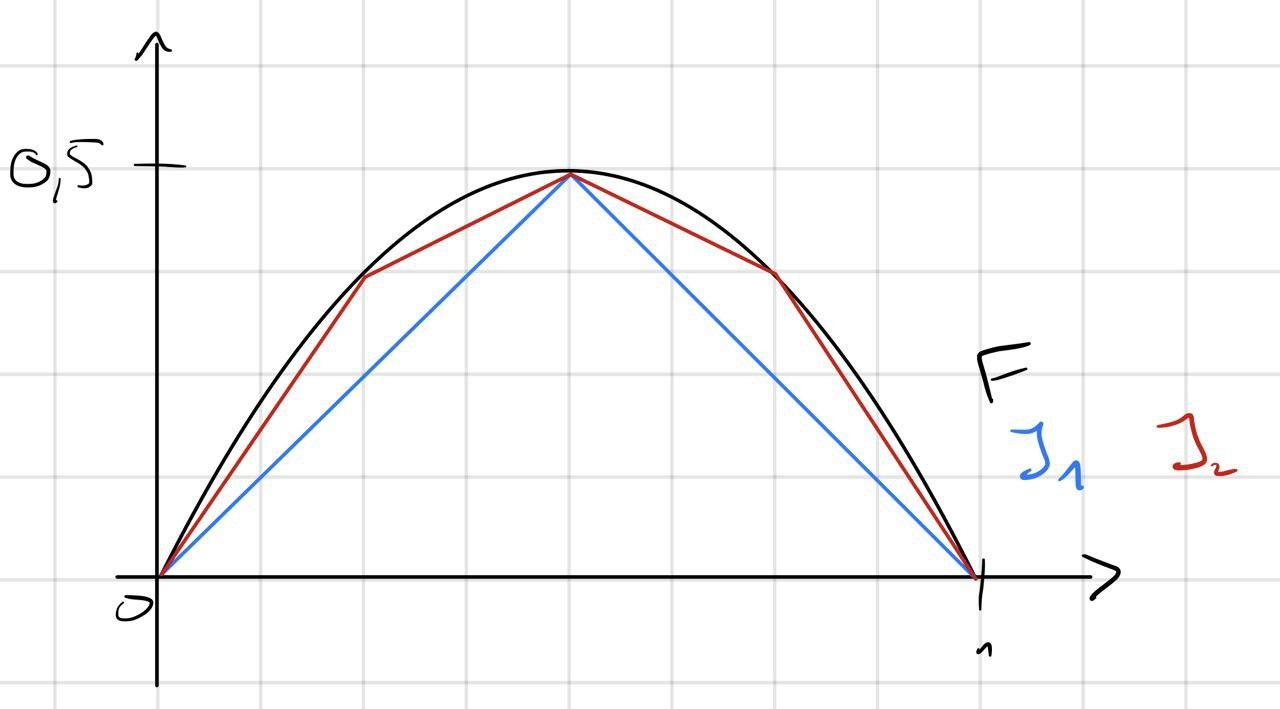
\includegraphics[width=5cm]{images/iii2_1.jpg} % iii2_1
\end{center}

Sei deshalb \(f_m: [0,2^{-m}] \rightarrow [0,2^{-2m-2}]\) definiert als \(f_m(x) = 2^{-m}x - x^2\)
und dessen lineare Interpolation \(h_m: [0,2^{-m}] \rightarrow [0,2^{-2m-2}]\) mit 
\[ h_m(x) \coloneqq \begin{cases}
    2^{-m-1}x, &x\in [0,2^{-m-1}), \\
    -2^{-m-1}x + 2^{-2m-1}, &x \in [2^{-m-1}, 2^{-m}].
\end{cases} \]

\begin{center}
    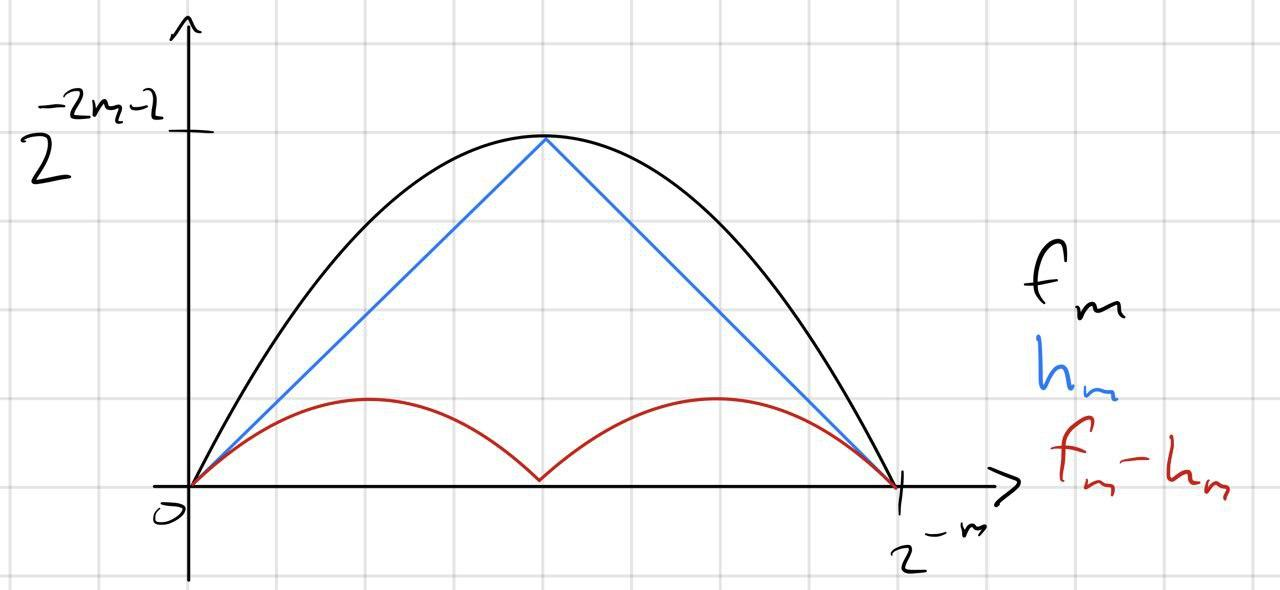
\includegraphics[width=5cm]{images/iii2_2.jpg} % iii2_2
\end{center}

Direktes Nachrechnen zeigt, dass 
\[ f_m(x) - h_m(x) = \begin{cases}
    f_{m+1}(x), &x\in [0, 2^{-m-1}), \\
    f_{m+1}(x - 2^{-m-1}), &x \in [2^{-m-1}, 2^{-m}].
\end{cases} \]

\textit{Zeige Fig. 2 aus Paper an Beamer}

\(F = f_0\) und \(I_1 = h_0\) implizieren, dass 
\[ F(x) - I_m(x) = f_m(x - \frac{j}{2^m}) \quad x\in [\frac{j}{2^m}, \frac{j+1}{2^m}] \]
und \(I_m = \sum_{k=0}^{m-1} H_k\) mit \(H_k : [0,1]\rightarrow \R\) gegeben durch 
\[ H_k(x) = h_k(x - \frac{j}{2^k}), \quad x\in [\frac{j}{2^m}, \frac{j+1}{2^m}]. \]

\begin{center}
    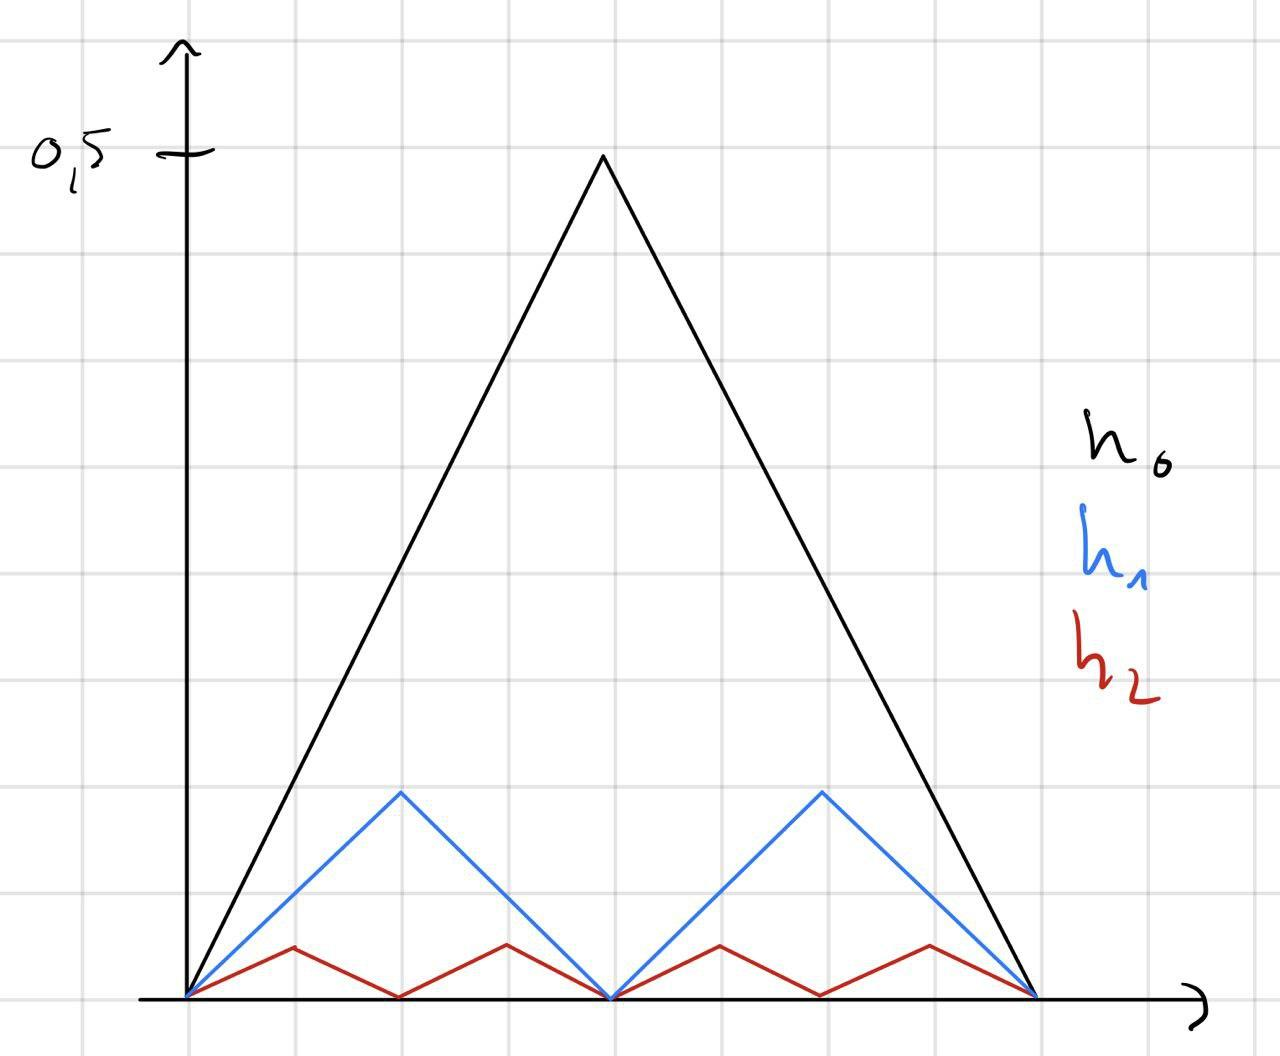
\includegraphics[width=5cm]{images/iii2_3.jpg} % iii2_3
\end{center}

Daraus folgt 
\[ \sup_{x\in [0,1]} |x^2 - (x - I_m(x)) | = \sup_{x\in [0,1]} |F(x) - I_m(x) | = \sup_{x\in [0, 2^{-m}]} |f_m(x)| = 2^{-2m-2}. \]

\textit{Hier verwenden wir das vorherige Lemma, 
der Approximationsfehler bleibt gleich in jedem Intervall.}

Aus der Sawtooth Konstruktion folgt, dass wir eine einfache Approximation der \(H_k\) finden 
durch ein neuronales Netzwerk mit zwei Neuronen pro Ebene 
sowie einem dritten Neuron, um die Approximation \(x - I_m(x)\) für \(x^2\) zu erreichen.

Sei \(s_k(x) \coloneqq 2^{-1}\rho(x) - \rho(x - 2^{-2k-1})\).
\begin{center}
    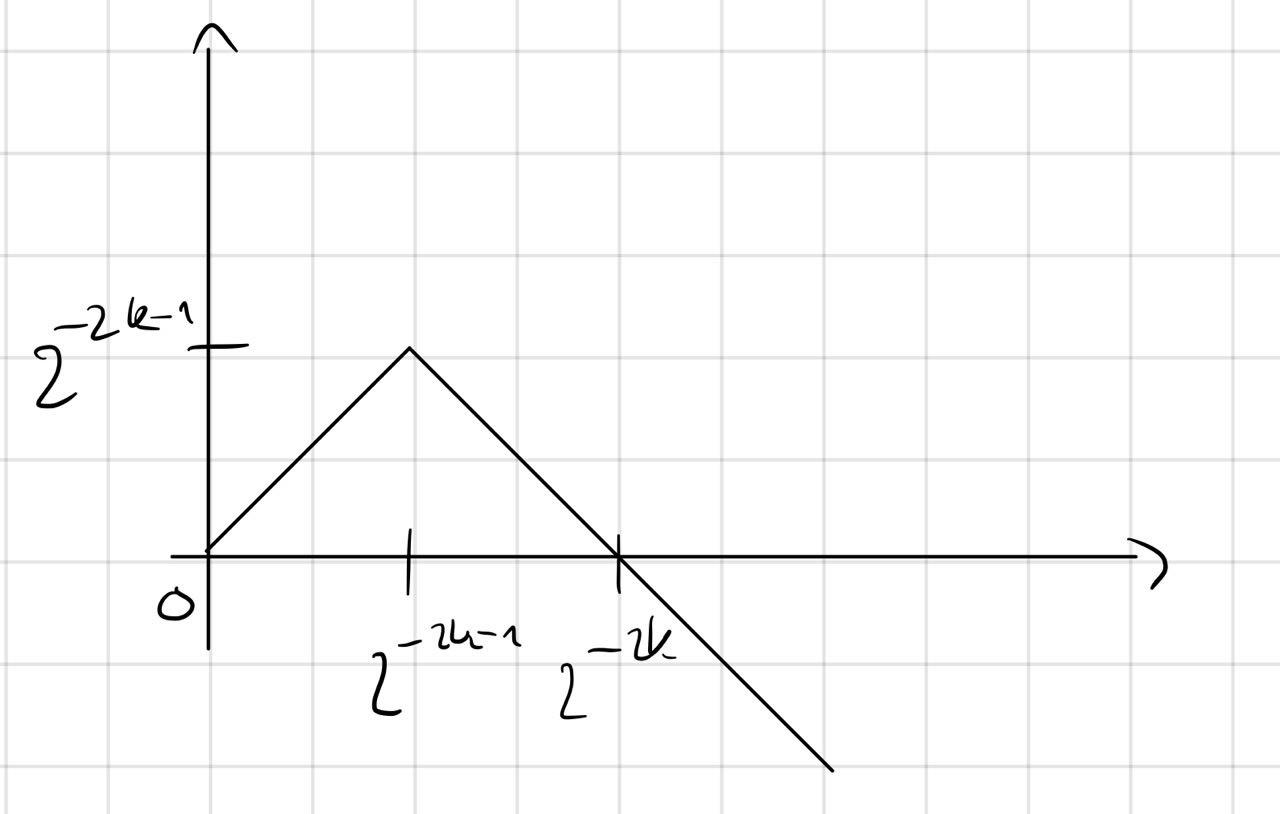
\includegraphics[width=5cm]{images/iii2_4.jpg} % iii2_4
\end{center}

\textit{Nun können wir jede dieser \(H_k\) Summen durch eine Netz Ebene approximieren 
und kommen so auf einen Fehler, der exponentiell schrumpft in der Netzwerklänge.}

\textit{Evtl. überspringen?}

Es gilt \(H_k = s_k \circ H_{k-1}\). Wir können ein Netzwerk \(x - I_m(x)\) wie folgt definieren: 
\(A_1 \coloneqq (1, 1, 1)^T \in \R^{3\times 1}, b_1 \coloneqq (0, -2^{-1}, 0)^T \in \R^3 \),
\[ A_l \coloneqq \begin{pmatrix}
    2^{-1} & -1 & 0 \\ 2^{-1} & -1 & 0 \\ -2^{-1} & 1 & 1
\end{pmatrix} \in \R^{3 \times 3}, b_l \coloneqq \begin{pmatrix}
    0 \\ -2^{-2l + 1} \\ 0
\end{pmatrix} \in \R^3 \]
sowie 
\(A_{m+1} \coloneqq (-2^{-1}, 1, 1) \in \R^{1 \times 3}, b_{m+1} = 0\).

Setzen wir \(W_l(x) \coloneqq A_l x + b_l\) und 
\[ \tilde{\Phi}_m \coloneqq W_{m+1} \circ \rho \circ W_m \circ \cdots \circ \rho \circ W_1, \]
bekommen wir durch direktes Nachrechnen \(\tilde{\Phi}_m(x) = x - \sum_{k=0}^{m-1} H_k(x)\). 
Der Fehler schrumpft exponentiell in der Netzwerklänge, \(\Phi_\varepsilon \coloneqq \tilde{\Phi}_{\lceil \log(\varepsilon^{-1})/2 \rceil}\) 
erfüllt die geforderten Eigenschaften.

\newpage
{\Large Proposition III.3}

Wir können o. B. d. A. annehmen, dass \(D \geq 1\) gilt. Für \(D < 1\) 
betrachten wir einfach das Netz, das für \(D=1\) konstruiert wird, welche die gleichen 
Eigenschaften erfüllt.

Die Argumentation basiert auf der Polarisationsformel 
\[ xy = \frac{1}{4} ((x+y)^2 - (x-y)^2). \]
Wir konstruieren zwei Quadrier-Netzwerke (Proposition III.2), 
die die Neuronen, die für die Summation der \(H_k\) verwenden, teilen 
sowie davor ein Layer, welches \((x,y)\) auf 
\((\frac{|x+y|}{2D}, \frac{|x-y|}{2D})\) 
abbilded sowie eine Ebene, die mit \(D^2\) multipliziert mit Gewichten, 
die durch \(1\) beschränkt sind. 
\textit{Den extra Schritt mit dem um \(D\) skalieren und zum Schluss wieder reskalieren 
machen wir, damit wir das Quadrierungsnetzwerk aus dem vorherigen Satz verwenden können.}

\textit{Matrizen auf den Folien kurz zeigen}

Baue hier ein Netzwerk \(\tilde{\Psi}_m\), 
welches folgendes erfüllt: 
\[ \tilde{\Psi}_m(x,y) = \tilde{\Phi}_m(\frac{|x+y|}{2D}) - \tilde{\Phi}_m(\frac{|x-y|}{2D}), \qquad(*) \]
wobei \(\tilde{\Phi}_m\) wie im vorherigen Beweis definiert ist.

Nun folgt 
\[ \sup_{(x,y) \in [-D,D]^2} |\tilde{\Psi}_m(x,y) - \frac{xy}{D^2} | 
= \sup_{(x,y) \in [-D,D]^2} |(\tilde{\Phi}_m(\frac{|x+y|}{2D}) - \tilde{\Phi}_m(\frac{|x-y|}{2D})) 
- ((\frac{|x+y|}{2D})^2 - (\frac{|x-y|}{2D})^2)| \] 
\[ \leq 2 \sup_{z\in [0,1]} |\tilde{\Phi}_m(z) - z^2| \leq 2^{-2m-1}. \qquad (**)\]

Setze nun \(\Psi_D(x) = D^2 x\) und wähle 
\(\Phi_{D,\varepsilon} \coloneqq \Psi_D \circ \tilde{\Psi}_{m(D,\varepsilon)} \), 
wobei \(m(D, \varepsilon) \coloneqq \lceil 2^{-1}(1+\log(D^2 \varepsilon^{-1})) \rceil \).
Dann folgt die Fehlerabschätzung aus \((**)\) und die geforderten Beschränkungen an 
die Breite, Länge und das Gewicht folgen aus der Konstruktion des Netzes zusammen mit Proposition III.2.

Weiter folgt \(\Phi_{D,\varepsilon}(0,x) = \Phi_{D,\varepsilon}(x,0) = 0\) direkt aus \((*)\).

\newpage

{\Large Lemma III.7}

\textit{Es gibt ein fundamentales Ergebnis aus der Lagrange Interpolation mit 
Tschebyscheff Punkten, welche folgendes garantiert.}
Satz: 
Für alle \(f\in \mathcal{S}_{[-1,1]}\), \(m\in\N\) existiert ein Polynom 
\(P_{f,m}\) mit Grad \(m\), sodass 
\[ ||f - P_{f,m}||_{L^\infty ([-1,1])} \leq \frac{1}{(m+1)!2^m} ||f^{(m+1)}||_{L^\infty ([-1,1])} \leq \frac{1}{2^m}. \]

Wir können \(P_{f,m}\) durch die Tschebyscheff-Basis darstellen: 
\[ P_{f,m} = \sum_{j=0}^m c_{f,m,j} T_j(x) \]
mit \(|c_{f,m,j}| \leq 2\) 
und den Tschebyscheff-Polynomen, die durch die Zweitermrekursion 
\[ T_k(x) = 2x T_{k-1}(x) - T_{k-2}(x), T_0(x) = 1, T_1(x) = x \]
definiert sind.
Weiter gilt, dass die Koeffizienten von \(T_k\) in der Monom-Basis 
durch \(3^k\) beschränkt sind. 
Also können wir \(P_{f,m} = \sum_{j=0}^m a_{f,m,j} x^j\) schreiben mit 
\[ A_{f,m} \coloneqq \max_{j=0,\ldots, m} |a_{f,m,j}| \leq 2(m+1)3^m. \] 

Wenn wir nun Proposition III.5 anwenden auf \(P_{f,m}\) mit \(m= \lceil \log(2/\varepsilon)\rceil\) 
und Approximationsfehler \(\varepsilon/2\), folgt die Behauptung durch
\[ C' m(\log(2/\varepsilon) + \log(m) + \log(|A_{f,m}|)) \leq C (\log(\varepsilon^{-1}))^2 \]
für eine Konstante \(C\).

\end{document}